\section{Model Evaluation}
\subsection{Model selection}
We use the Bayes factor $B_{1, 2}$ to perform a model comparison between the model $1$ (without seniority) and the model $2$ (with seniority)
\begin{equation*}
B_{1, 2}=\frac{p \left(y \mid m=1 \right)}{p \left(y \mid m=2 \right)}=\frac{\int p\left(y \mid \theta, m=1 \right) \pi_{m=1} \left(\theta \right) d \theta}{\int p\left(y \mid \theta, m=2 \right) \pi_{m=2} \left(\theta \right) d \theta}
\end{equation*}
where we compute the marginal likelihoods $p \left(y \mid m \right)$ using the Bridge estimator
\begin{equation*}
\hat{p}=\frac{\sum_{t} \pi\left(\theta^{(1, t)}\right) p\left(y \mid \theta^{(1, t)}\right) h\left(\theta^{(1, t)}\right)}{\sum_{t} \pi\left(\theta^{(2, t)}\right) h\left(\theta^{(2, t)}\right)}
\end{equation*}
where $\theta_{t}^{(1)} \sim \pi(\theta)$ are random samples simulated from the prior and $\theta_{t}^{(2)} \sim \pi(\theta \mid y)$ are simulated from the posterior. As a rule of thumb we choose $h(\theta)=\pi(\theta)^{-1} p \left(y \mid \theta \right)^{-1 / 2}$ so that the bridge estimator simplifies to
\begin{equation*}
\hat{p}=\frac{\sum_{t} p\left(y \mid \theta^{(1, t)}\right)^{1 / 2}}{\sum_{t} p\left(y \mid \theta^{(2, t)}\right)^{-1 / 2}}
\end{equation*}
The estimated Bayes factor $\hat{B}_{1, 2}$ has the order of magnitude of $10^{5}$ and does not vary upon multiple computations, providing substantial evidence in favour of the model without seniority covariates than the model with.

\begin{figure}[ht!] \centering
\begin{subfigure}[b]{0.45\textwidth} \centering
   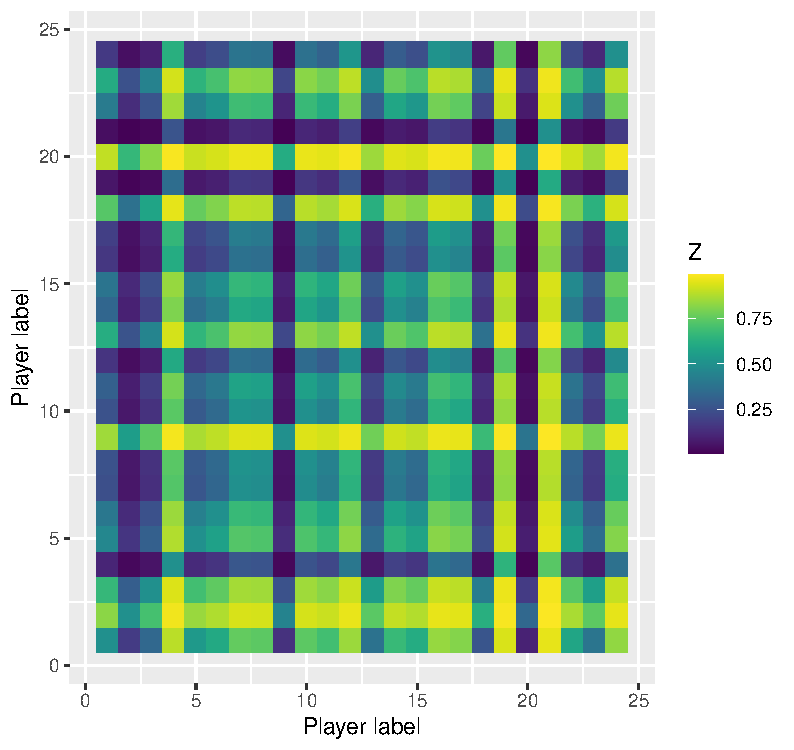
\includegraphics[width=1\linewidth]{heat_one}
   \caption{Model 1 pairwise skill comparisons} \label{fig:6a}
\end{subfigure}
\begin{subfigure}[b]{0.45\textwidth} \centering
   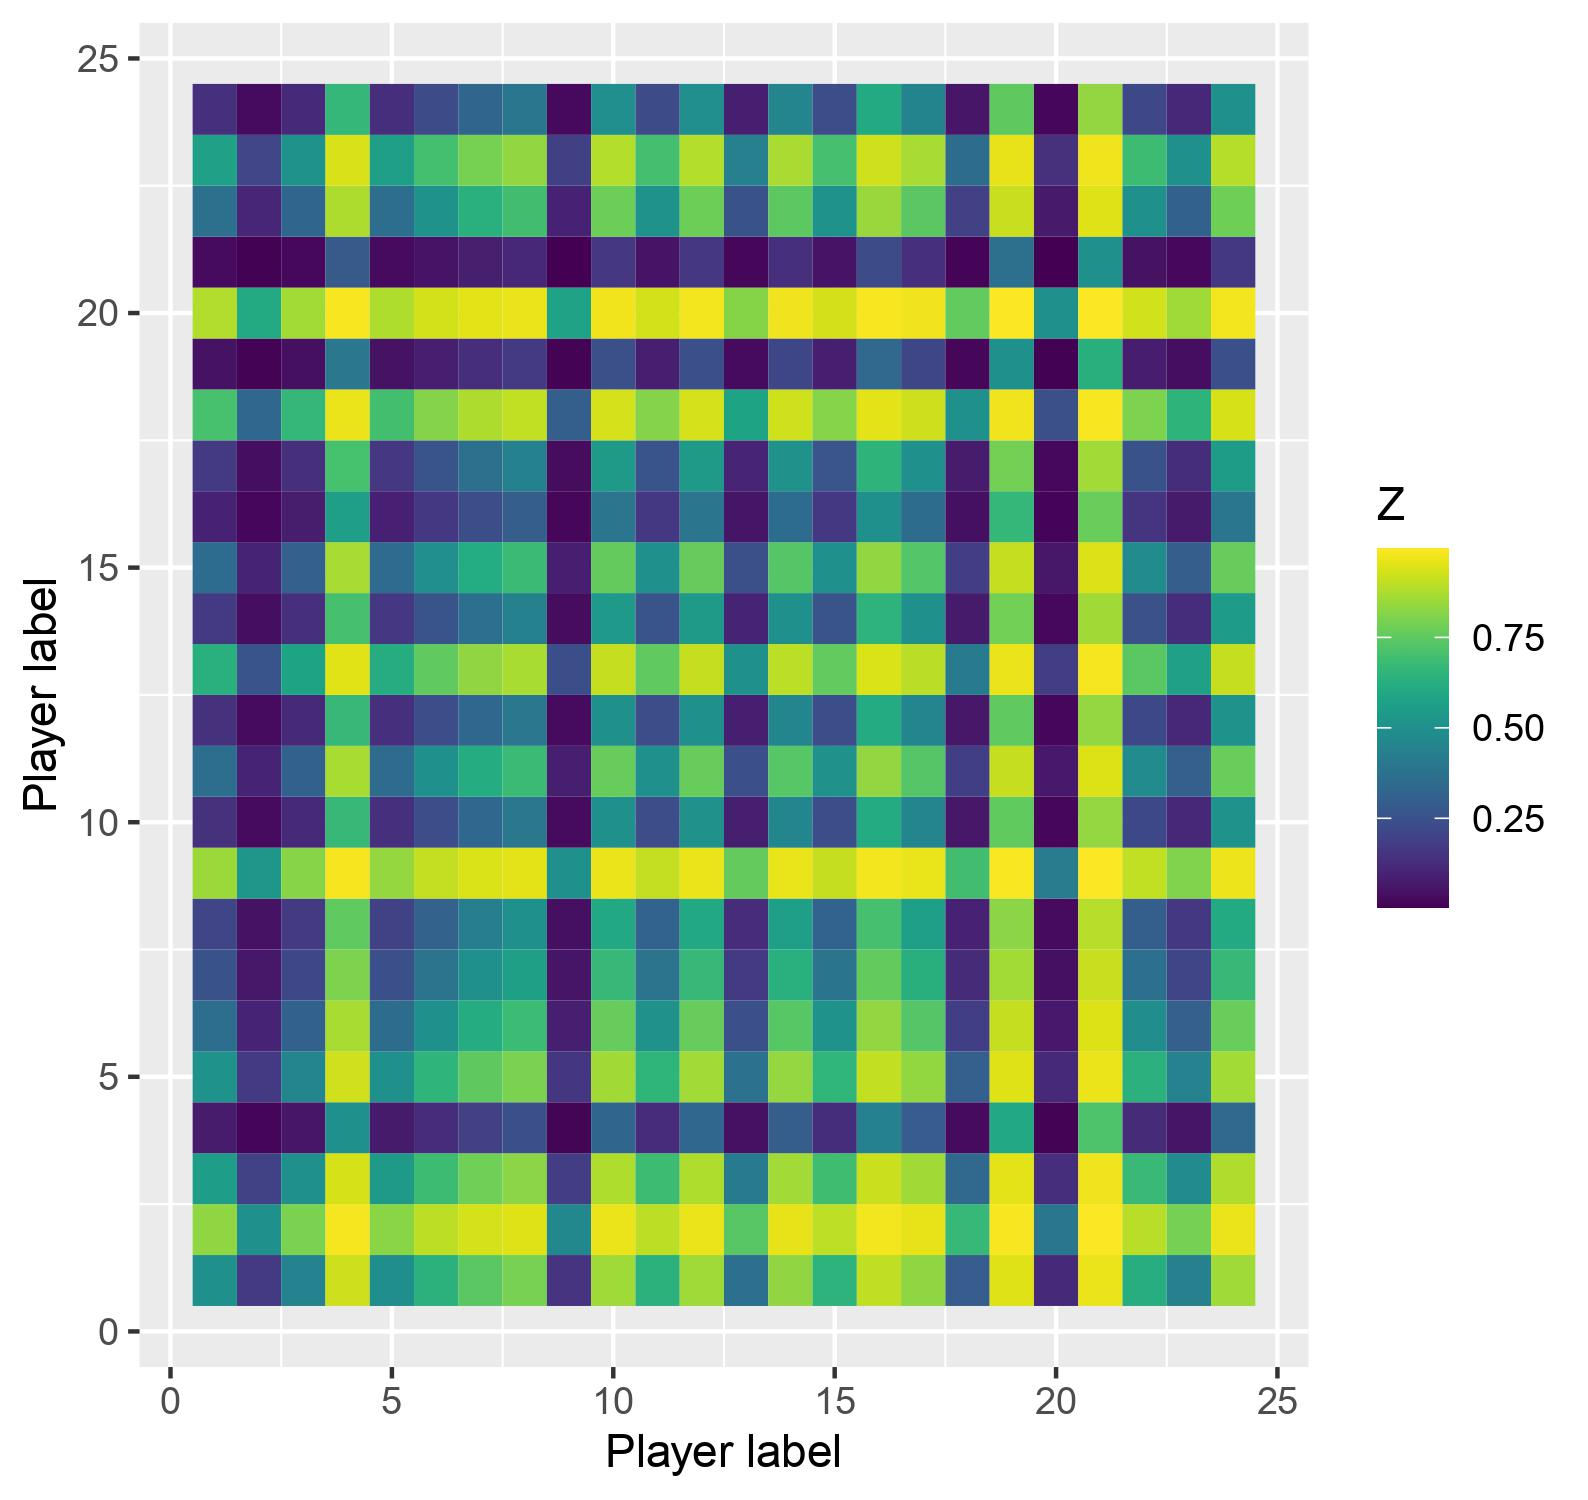
\includegraphics[width=1\linewidth]{heat_two}
   \caption{Model 2 pairwise skill comparisons} \label{fig:6b}
\end{subfigure} \hspace{1em}
\caption{Pairwise comparisons of the relative skills of the players. The value in the heat map indicates the probability of the row player winning in a game against the column player.}
\label{fig:6}
\end{figure}

\subsection{Player skills}
We report the posterior mean and the HPD intervals of parameters from model one below. A similar summary is reported in Appendix~\ref{app:1}. From the posterior mean, we can conclude that players $21, 19, 4$ have the strongest skills, whereas players $20, 2, 9$ have the weakest. We perform a comparison of the relative skills of each pair $\{i, j\}$ of players in the dataset by considering the probability that $i$ wins in the game involving only the two players (Figure~\ref{fig:6}). The sign convention adopted here is that the value in the heat map indicates the probability that the row player wins in a game against the column player.
\begin{equation*}
\operatorname{Pr}\{i~\text{win}\}= \frac{\exp (\hat{\lambda}_{o_{i}})}{\exp (\hat{\lambda}_{o_{i}}) + \exp (\hat{\lambda}_{o_{j}})}
\end{equation*}

\begin{table} \center
\begin{tabular}{cccc}
\text { Param. } & \text { Post. Mean } & \text { HPD interval } & \text { ESS } \\
\hline
$\lambda_{1}$ & -0.67 & (-2.18, 0.85) & 1132 \\
$\lambda_{2}$ & -2.31 & (-4.09, -0.44) & 884 \\
$\lambda_{3}$ & -1.35 & (-3.68, 0.52) & 1000 \\
$\lambda_{4}$ & 1.35 & (-0.11, 2.97) & 1000 \\
$\lambda_{5}$ & -0.45 & (-1.41, 0.42) & 1000 \\
$\lambda_{6}$ & -0.11 & (-1.75, 1.50) & 1000 \\
$\lambda_{7}$ & 0.76 & (0.07, 1.51) & 1000 \\
$\lambda_{8}$ & 0.30 & (-0.54, 1.13) & 1230 \\
$\lambda_{9}$ & -2.25 & (-3.58, -1.01) & 1000 \\
$\lambda_{10}$ & 0.39 & (-0.19, 1.05) & 1000 \\
$\lambda_{11}$ & 0.20 & (-0.51, 0.94) & 1000 \\
$\lambda_{12}$ & 0.90 & (-0.26, 1.81) & 1000 \\
$\lambda_{13}$ & -0.82 & (-2.08, 0.45) & 960 \\
$\lambda_{14}$ & 0.09 & (-1.15, 1.44) & 1000 \\
$\lambda_{15}$ & -0.26 & (-1.07, 0.40) & 1000 \\
$\lambda_{16}$ & 1.17 & (-0.23, 2.56) & 1000 \\
$\lambda_{17}$ & 0.91 & (-0.28, 2.04) & 1077 \\
$\lambda_{18}$ & -1.44 & (-3.41, 0.05) & 798 \\
$\lambda_{19}$ & 2.03 & (0.79, 3.36) & 1000 \\
$\lambda_{20}$ & -2.36 & (-4.57, -0.57) & 825 \\
$\lambda_{21}$ & 2.91 & (0.23, 6.02) & 879 \\
$\lambda_{22}$ & -0.19 & (-1.84, 1.44) & 1000 \\
$\lambda_{23}$ & -0.97 & (-3.05, 1.26) & 1000 \\
$\lambda_{24}$ & 0.81 & (-0.42, 2.12) & 1000 \\
$olpr$ & -44.39 & (-52.62, -36.49) & 1000 \\
$ollk$ & -161.1 & (-168.27, -153.29) & 1000 \\
\end{tabular}
\caption{Summary of the posterior mean, HDP intervals and the ESS from model one}
\end{table}

\subsection{A Simple Example}
Consider a simple example where game $68$ involving players $s=\{4, 7, 11, 5, 10, 14, 15, 13, 9\}$ was replayed (i.e. with the same players and same seniority values), we are interested in the probability that player $7$ wins. We estimate this by summing the probabilities of all $7!$ permutations where player $7$ comes at the top
\begin{equation*}
  \sum_{o_{1}=7} E_{\lambda, \beta \mid model} \left[ \operatorname{Pr}\{O=o \mid \lambda, \beta\} \right] \quad \text{where} \quad O \in \mathcal{P}_{s}
\end{equation*}

The marginals are estimated using the Bridge estimator. In model one without seniority covariates, the probability is $17.4\%$ and is stable upon repeated runs of the bridge estimation. With model two, when the seniority covariates are added, the probability that player $7$ wins drops to $4.1\%$, indicating that seniority has non-trivial effects on the outcomes. Both estimates are stable upon multiple runs of the bridge estimator.
